\section{Compact whole-word repair atlases}
\label{sec:repair-atlases}

Let $\D$ be the protected polytopal supercode from \Cref{thm:protected-supercode}.  For a nonempty word $\sigma$, define its complete closed carrier
\[
 K_\sigma=Q\cap\bigcap_{i\in\sigma}P_i.
\]
Using the closed carrier rather than only the open atom ensures that threshold and lower-dimensional copies are included.

\begin{theorem}[Compact whole-word repair atlas]
\label{thm:repair-atlas}
Let $\sigma\notin\C$ be nonempty.  If $K_\sigma\ne\varnothing$, then there is a finite family
\[
 \{(R_r,\rho_r)\}_{r=1}^{N_\sigma}
\]
such that:
\begin{enumerate}[label=\textup{(\roman*)}]
\item $\rho_r\in\C$ and $\sigma\subsetneq\rho_r$;
\item $R_r$ is a full-dimensional compact polytope with
\[
 R_r\Subset\operatorname{int}Q\cap\bigcap_{i\in\rho_r}U_i;
\]
\item the relative interiors cover the complete carrier,
\[
 K_\sigma\subseteq\bigcup_r\operatorname{int}R_r;
\]
\item every point of $K_\sigma$ is assigned at least one complete source word strictly above $\sigma$.
\end{enumerate}
The finitely many words in $\D\setminus\C$ admit one finite combined atlas.
\end{theorem}

\begin{proof}
Because $P_i\Subset U_i$ for all $i\in\sigma$, the compact set $K_\sigma$ lies in
\[
 \operatorname{int}Q\cap\bigcap_{i\in\sigma}U_i.
\]
For $x\in K_\sigma$, let $\rho(x)$ be its source word.  Then $\sigma\subseteq\rho(x)$.  Since $\sigma$ is absent from $\C$, the containment is strict.  The open set
\[
 \operatorname{int}Q\cap\bigcap_{i\in\rho(x)}U_i
\]
contains $x$, so it contains a full-dimensional compact polytope $R_x$ with $x\in\operatorname{int}R_x$.  The interiors of these $R_x$ form an open cover of the compact carrier $K_\sigma$.  A finite subcover yields the atlas.

There are finitely many unwanted words, so the union of their finite atlases is finite.
\end{proof}

\begin{corollary}[One-label local deletion]
For each patch choose any index $j_r\in\rho_r\setminus\sigma$ and define
\[
 \widehat P_j
 =\conv\left(P_j\cup\bigcup_{r:j_r=j}R_r\right).
\]
Leaving the $P_i$ with $i\in\sigma$ unchanged eliminates the word $\sigma$, keeps every enlarged polytope inside its source neuron, and preserves all protected target witnesses.
\end{corollary}

\begin{proof}
Every set used to enlarge $P_j$ is compactly contained in the open convex set $U_j$, so its finite convex hull remains in $U_j$.  A point in all $P_i$ for $i\in\sigma$ belongs to $K_\sigma$ and hence to the interior of some $R_r$, which activates an index $j_r\notin\sigma$.  Protected positive memberships cannot be lost; a protected inactive witness cannot enter $\widehat P_j\subset U_j$.
\end{proof}

\begin{figure}[t]
\centering
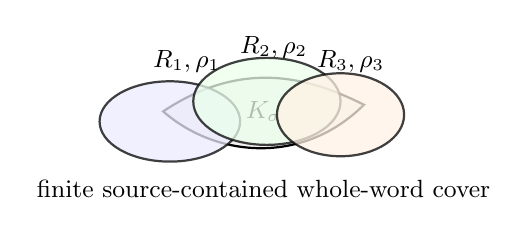
\begin{tikzpicture}[scale=.85,font=\small]
\draw[thick,fill=gray!10] (0,0) .. controls (1.2,.8) and (2.2,.5) .. (3,.1) .. controls (2.1,-.8) and (.8,-.7) .. cycle;
\node at (1.5,0) {$K_\sigma$};
\draw[thick,fill=blue!8,opacity=.75] (.1,-.15) ellipse (1.05 and .6);
\draw[thick,fill=green!8,opacity=.75] (1.55,.15) ellipse (1.1 and .65);
\draw[thick,fill=orange!10,opacity=.75] (2.65,-.05) ellipse (.95 and .62);
\node at (.35,.75) {$R_1,\rho_1$};
\node at (1.65,.95) {$R_2,\rho_2$};
\node at (2.8,.75) {$R_3,\rho_3$};
\node at (1.5,-1.15) {finite source-contained whole-word cover};
\end{tikzpicture}
\caption{A complete unwanted carrier is compact.  Source words strictly above it provide an open cover by whole-word neighborhoods; compactness yields a finite repair atlas.}
\label{fig:repair-atlas}
\end{figure}

\begin{remark}[Elimination of local analytic infinity]
No positive separation or nondegeneracy is assumed.  Even if a forbidden carrier accumulates on many source boundaries, compactness produces finitely many full-dimensional source-contained charts.  Thus zero margin does not force an infinite local atlas.
\end{remark}

\begin{remark}[Why the theorem stops short]
The corollary eliminates one current carrier by assigning patches to selected neurons.  Applying many such operations, or convexifying all occurrences of a repeated neuron independently, may create new mixed-hull intersections elsewhere.  The existence of a finite atlas is not the existence of one simultaneous global convex attachment.
\end{remark}
